
\documentclass{article}

\usepackage{amssymb,amsmath}

\usepackage{graphicx}

\begin{document}

\section{Risk Model}

Risk is modelled as a function, $\mathbb{R}^3 \rightarrow [0, 1]$ which is use
to determine the risk at every $(x, y, z)$ location within the search space. In
order to determine risk in 3-space, we obtain a 2-D risk model which models the
risk at the minimum altitude. This function $R_0 : \mathbb{R}^2 \rightarrow [0,
1]$ determines what the risk would be at the minimum altitude. This is assumed
to be given to the algorithm \emph{a priori} or can be determined at any time
during the iteration of the algorithm. This ground risk, $R_0$, is modelled as
a lookup table rather than a combination of basis functions in order to give a
more generic model for risk that can be used in any use case of the algorithm.
To determine the 3-D risk, $R(x, y, z)$, we perform an exponential decay on the
given ground risk value, $R_0(x, y)$. 3D risk is defined as follows:

$$ R(x, y, z) = R_0(x, y) \cdot \exp{\left(-\frac{z^2}{K \cdot R_0(x,
y)^2}\right)}$$

Even though risk in 3D is evaluated and is not simply a lookup table, one can
be used instead. This representation for 3D risk is ideal for modelling fires,
detection by hostile agents, or any stimuli that would decrease monotonically
as the altitude increases.

For the experiments, we have used nine different scenes for the representation
of the ground risk, $R_0$. To generate these scenes, we used the diamond-square
algorithm~\cite{DBLP:journals/cacm/FournierFC82} to generate random terrain
maps that have values from zero to one.  The diamond-square algorithm generates
realistic random risk scenes that represent the 2D ground level risk as
anticipated. Random terrain maps have also been used
in~\cite{DBLP:conf/icra/MurphyN11} to represent random risk for path planning
problems. A heat-map showing a random terrain map generated with the diamond
square algorithm is shown in Fig~\ref{fig:risk}.

\begin{figure}[h]

    \centering

    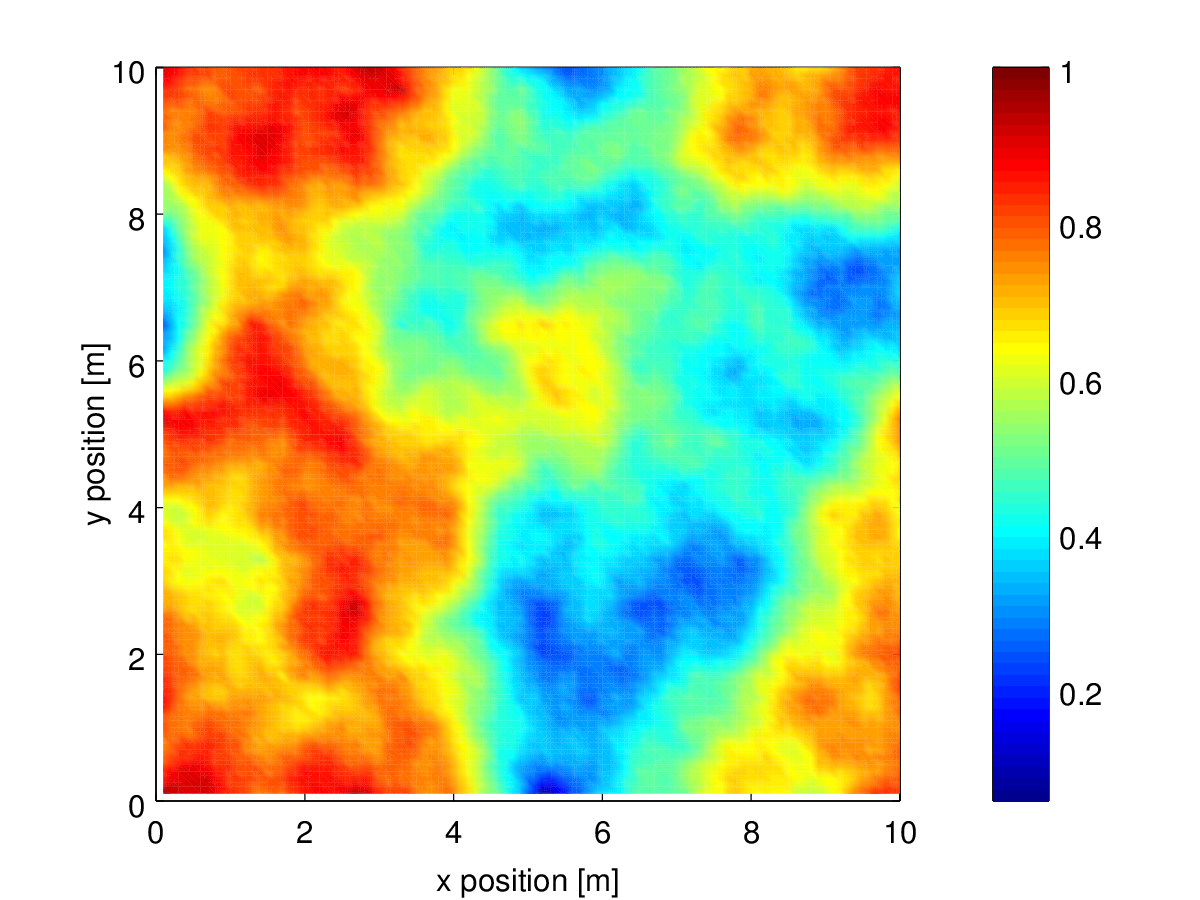
\includegraphics[width=1.0\columnwidth]{tasefigs/risk.png}

    \caption{A visualization of the ground risk, $R_0$}

    \label{fig:risk}

\end{figure}

\section{2D Planning}

Quadrotors use a very simple, reactive rule to determine where to move that has
extremely emergent properties.  Given a map, $M$, quadrotors move to areas with
a combination of the largest uncertainty, $\Upsilon$, and the lowest risk, $R$.
Our implementation uses a cost surface that is shared between members of the
swarm. Since the quadrotors update this cost surface as they move around it,
the cost surface is used as the mode of communication between the quadrotors.
This cost surface removes the need for the agents to have any peer to peer
communication and also removes the need for any agent to have perfect
information about the swarm.

For a quadrotor to determine a new heading, the agent samples costs from the
surface around the edge of its sensor foot print. It then moves in the
direction of the smallest cost. One it has moved, the agent updates the
measurements for the uncertainty grid, $\Upsilon$ for the area that was just
covered in by the sensor foot print. This uncertainty update happens
iteratively in the swarm, so the quadrotors left the plan their movements have
an updated grid before they determine a new heading.

The cost surface, $\Gamma$, is made up of a combination of the uncertainty
grid, $\Upsilon$ and the risk surface of the region. More formally, assume that
there is a function $\delta : \mathbb{R}^2 \rightarrow \mathbb{R}$ which is
used to combine the uncertainty and risk into one metric. This is assumed to be
a user defined function which may change from application to application. The
cost surface is then defined as,

$$\Gamma(x, y) = \delta(\Upsilon(x, y), R(x, y))$$

For our implementation we defined $\delta$ as,

$$\delta(\upsilon, r) = \max{\Upsilon} - \upsilon + 100 \cdot r$$

An instance of the uncertainty surface, $\Upsilon$, is shown in
Fig~\ref{fig:unc} where the $x, y$ coordinate represents the 2D position within
the workspace and the color represents the level of uncertainty. Notice the two
dark blue ellipses with low uncertainty. That is the current sensor footprint
of the quadrotors at the time at which the snapshot was taken.
Fig.~\ref{fig:cost} shows a snapshot of the cost surface which is created by
combining the risk surface shown in Fig.~\ref{fig:risk} and the uncertainty
surface shown in Fig.~\ref{fig:unc} using the $\delta$ combination function
used in our implementation.

\begin{figure}[h!]

    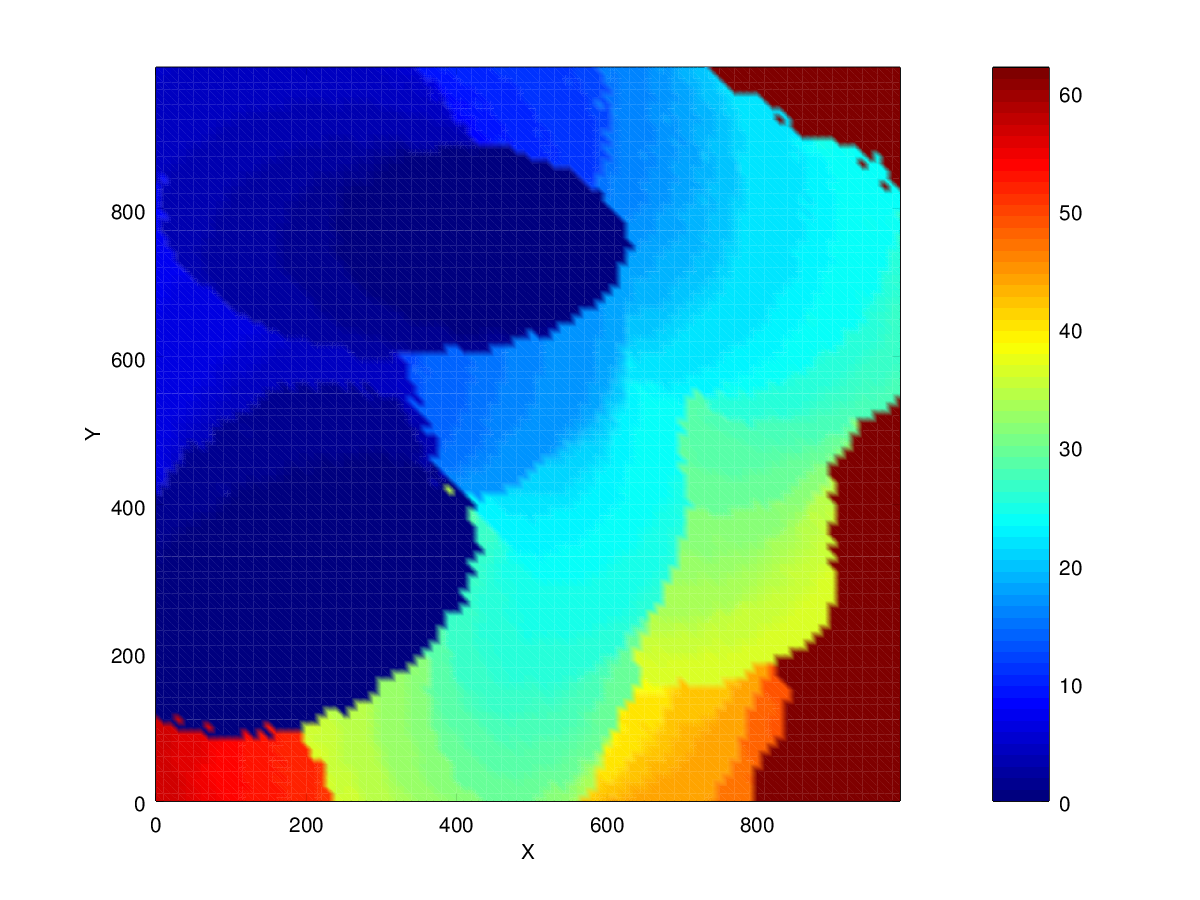
\includegraphics[width=1\columnwidth]{tasefigs/uncertainty.png}

    \caption{Uncertainty surface where red represents higher uncertainty}

    \label{fig:unc}

\end{figure}

\begin{figure}[h!]

    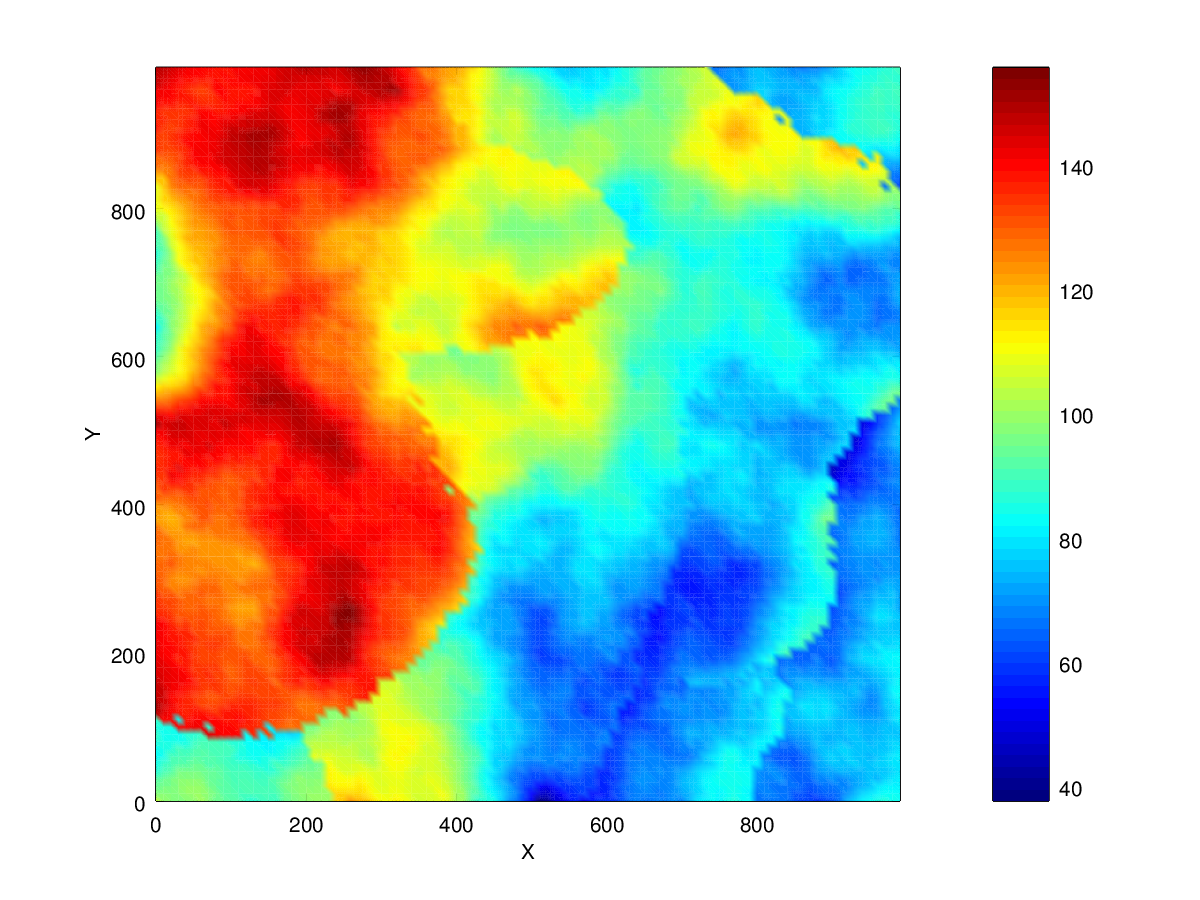
\includegraphics[width=1\columnwidth]{tasefigs/costsurf.png}

    \caption{Cost surface which is a combination of the uncertainty surface
    in Fig.~\ref{fig:unc} and Fig.~\ref{fig:risk} where red represents higher
cost}

    \label{fig:cost}

\end{figure}

\bibliographystyle{IEEEtran} \bibliography{mp,plaku,quads,relatedwork}

\end{document}
